\chapter{Nola testatu Express aplikazioak}

Kapitulu honetan Express aplikazio bat testeatzen ikasiko dugu. Hemen proba unitarioak erabiliko ditugu soilik (proba funtzionalak, integrazio probak, erregresio probak etab. alde batera utziz). Eskarmentua baduzu Javaz landutako proba unitarioekin (\textit{JUnit framework}a erabiliz), bide luze bat jada aurreratu duzu: express-en egindako aplikazioak berdin testeatu daitezke, baina beste framework pare baten laguntzarekin: \index{Jest} eta \index{SuperTest}.

\begin{enumerate}

    \item Gauzak probatzen hasteko, express aplikazio sinple bat sortuko dugu:

\begin{lstlisting}[language=JavaScript,numbers=none]
$ express --view=ejs express-test
$ cd express-test
$ npm install    
\end{lstlisting}

\item 
    jest, supertest eta cross-env paketeak instalatu

(-D aukerak devDependencies - alegia, garatze-garaiko mendekotasunak- instalatzen ditu. Pakete horiek ez dira beharrezkoak aplikazioa martxan jartzeko edota erabiltzeko, soilik testeatzeko/garatzeko erabiliko ditugu)

\begin{lstlisting}[language=JavaScript,numbers=none]
$ npm install  -D jest supertest
$ npm install -g cross-env
\end{lstlisting}

\item 
package.json fixategian hau txertatu (node aplikazioak testeatu nahi ditugula esaten ari gara hemen, eta node\_modules karpetaren barruan dagoena ez dugula testeatu nahi)

\begin{lstlisting}[language=JavaScript,numbers=none]
....
"jest": {
 "testEnvironment": "node",
 "coveragePathIgnorePatterns": [
   "/node_modules/"
 ] 
 }...
\end{lstlisting}

Gutxi gora-behera horrelako package.json bat lortuko duzu:


\begin{figure}[ht]
	\centering
\begin{tikzpicture}
\node[anchor=south west,inner sep=0] (image) at (0,0)
   {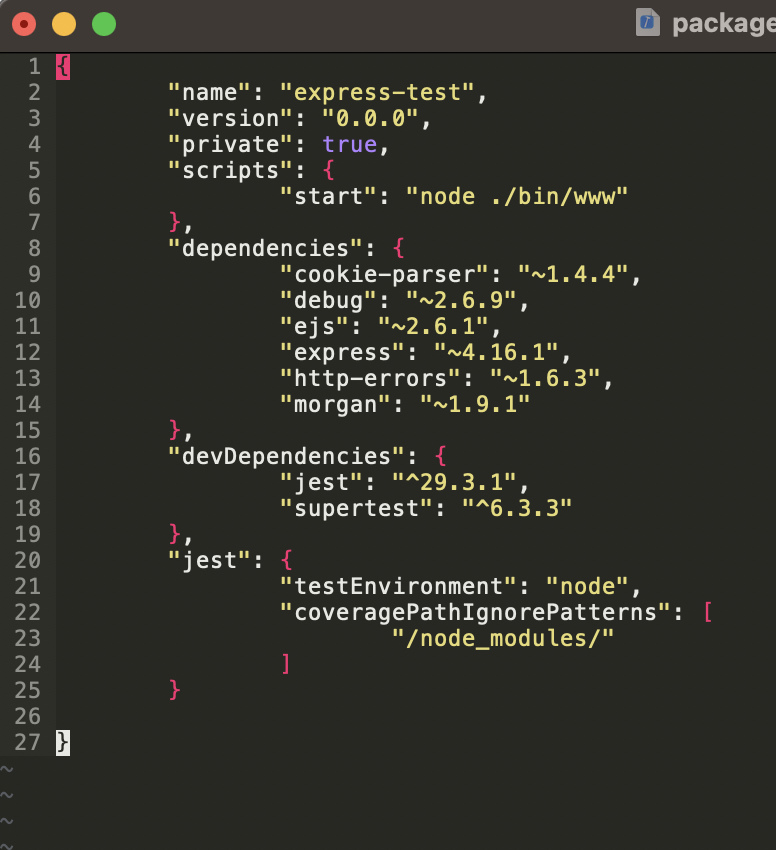
\includegraphics[trim=0cm 0cm 0cm 0cm, clip=true, width=0.75\textwidth]{img/testing/testing_package_json.png}};
\end{tikzpicture}
\caption{Testing: package json.}
\label{fig:testing-package-json}
\end{figure}


\item 
Jarraian, routes/users.js ezabatu eta routes/index.js fitxategiaren edukia Gist honen edukiarekin ordezkatu:

\href{https://gist.github.com/juananpe/8aa0cd571f07df8f278015ec476d3ecf}{https://gist.github.com/juananpe/8aa0cd571f07df8f278015ec476d3ecf}


Bertan, horrelako objektuak gorde (send), aldatu (update) eta ezabatzeko (destroy) rutak prestatu ditugu:

\begin{lstlisting}[language=JavaScript,numbers=none]
    const fakeDB = [
 {
   id: Math.floor(Math.random() * 100),
   email: "test@example.com",
 },
];
\end{lstlisting}

\begin{itemize}
    \item 

Oharra: adibidea errazteko, fakeDB objektua sortu dugu, mongoDB datubase bat simulatzen duena, array baten bidez.
\item 
Oharra: bi lerro hauek ezabatu app.js fitxategitik: 

\begin{lstlisting}[language=JavaScript,numbers=none]
var usersRouter = require('./routes/users');
....
app.use('/users', usersRouter);
\end{lstlisting}


\end{itemize}

\item 
package.json fitxategian, scripts atala horrela moldatu:


\begin{verbatim}
    
 "scripts": {
   "start": "node ./bin/www",
   "test": "cross-env NODE_ENV=test jest"
 },

\end{verbatim}


Oharra: NODE\_ENV bidez testeatzeko ingurune batean ari garela zehazten ari gara. Besteak beste 404 erroreak baldin badaude eta test ingurunean bagaude, orduan errorearen zergatia bistaratzen duen traza bat agertuko zaigu (traza horiek ez dira agertu behar production ingurunean, segurtasunaren aldetik informazio gehiegi - eta pribatua- ematen dutelako)


\item 
Aplikazioa martxan jarri:

\begin{verbatim}
cross-env PORT=4444 DEBUG="express-test:*" nodemon start    
\end{verbatim}


eta probatu ondo dabilela (eskuz, testak oraindik ez ditugu prestatu eta)

Zehazki, http://localhost:4444/ bidean, erantzun hau jaso beharko genuke:


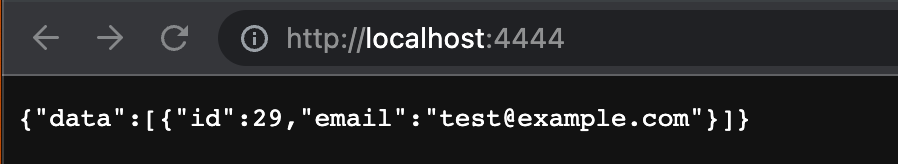
\includegraphics[width=0.75\textwidth]{img/testing/testing_view_index.png}

Berriz, POST \textbf{/send} endpoint-era eginez gero:

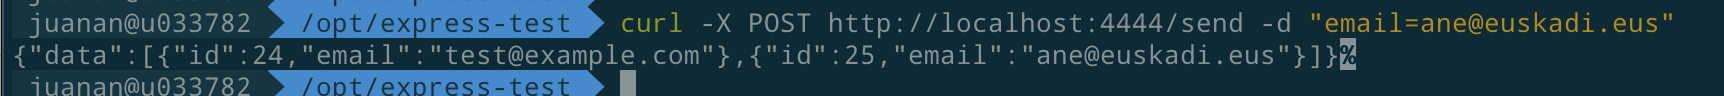
\includegraphics[width=0.75\textwidth]{img/testing/testing_post.png}

PUT endpoint-a probatzeko:

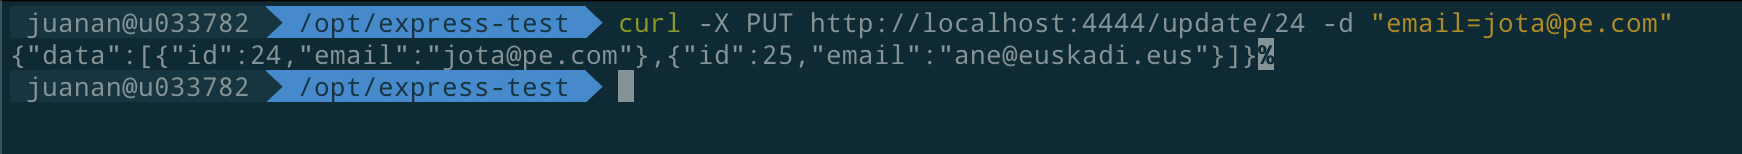
\includegraphics[width=0.75\textwidth]{img/testing/testing_put.png}


eta DELETE endpoint-a probatzeko:

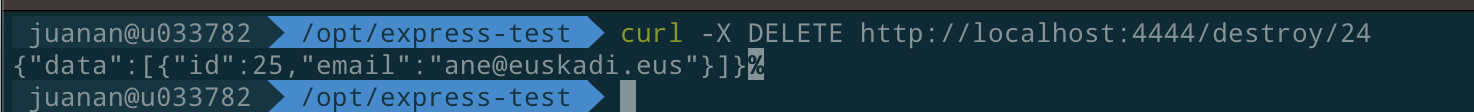
\includegraphics[width=0.75\textwidth]{img/testing/testing_delete.png}

\item 
Dena ondo doala probatu ostean, zerbitzaria eten eta berriro martxan jarri

\item 
Sortu \textbf{tests} karpeta eta bertan fitxategi hau:

\begin{lstlisting}[language=JavaScript,numbers=none]
    /* server.test.js */

const request = require('supertest');
const PORT = process.env.PORT || 4444;
const url = `http://localhost:${PORT}`


describe('Testing index', () => {
   it('GET /', async () => {
       const res = await request(url).get('/');
       expect(res.statusCode).toBe(200);
       expect(res.type).toBe('application/json');
       expect(res.type).toMatch(/json/);
   });
   // hurrengo it()
});

\end{lstlisting}


\textbf{Azalpena:}

\begin{enumerate}
    \item lehenengo 3 lerroetan supertest paketea inportatu ondoren, gure aplikazioarekin lotzen dugu. 
\item jarraian describe() funtzioak test multzo (test suite) bat deskribatzen du. describe baten barruan hainbat it() (test) funtzio izan ditzakegu. Baina momentzu ez dugu ezer probatu. Berez, jarraian datozen funtzioekin egingo ditugu testak.
\item get('/') funtzioak GET request bat egingo du / bidera. Erantzuna res (response) objektuan dator. 
\item behin res (erantzuna) dugula, barruan dagoen objektuen atributuak espero ditugun balioen kontra konparatuko ditugu expect() funtzioekin. Adibidez, GET / egin ondoren HTTP status code = 200 izatea espero dugu (gogoratu HTTP/200 = OK)
\item toBe(), toMatch, etab. expect() objektuaren metodoak dira. Gainontzeko metodo guztiak ezagutzeko, botaiozu begirada bat URL honi: https://jestjs.io/docs/expect 

\end{enumerate}


\item 
Exekutatu testak 
(Oharra: jest komandoak *.test.js bilatu eta exekutatuko ditu, automatikoki)
\begin{verbatim}
$ npm test    
\end{verbatim}

Dena ondo badoa, hau ikusiko duzu:

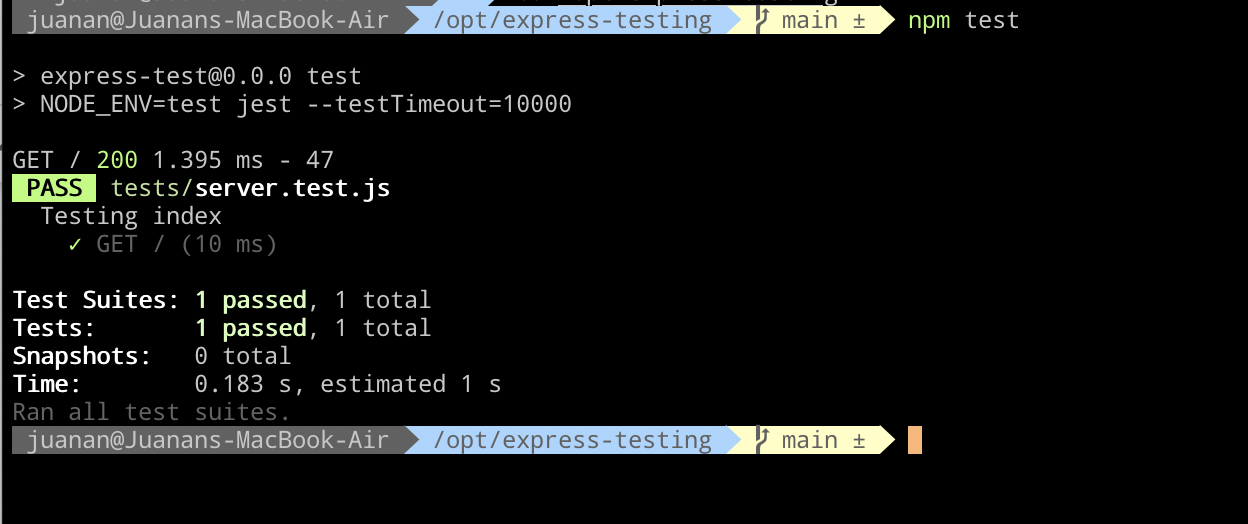
\includegraphics[width=0.75\textwidth]{img/testing/testing_npm_test.png}

\item 
Aurreko kode zatian, "//hurrengo it()" komentarioaren ondoren, hau sartu:

\begin{lstlisting}[language=JavaScript,numbers=none]
    it("POST /send", async () => {
   const res = await request(url).post("/send")
       .send({
           email: 'janire@example.com'
       });


   expect(res.type).toMatch(/json/)
   expect(res.statusCode).toBe(201)
   expect(res.body.data.length).toBe(2)
   expect(res.body.data[0].email).toMatch("test@example.com")
   expect(res.body.data[1].email).toMatch("janire@example.com")
})
\end{lstlisting}


Eta exekutatu berriro test multzoa, horrela:
\begin{verbatim}
$ npm test    
\end{verbatim}

Dena ondo badoa hurrengoa jaso beharko zenuke:

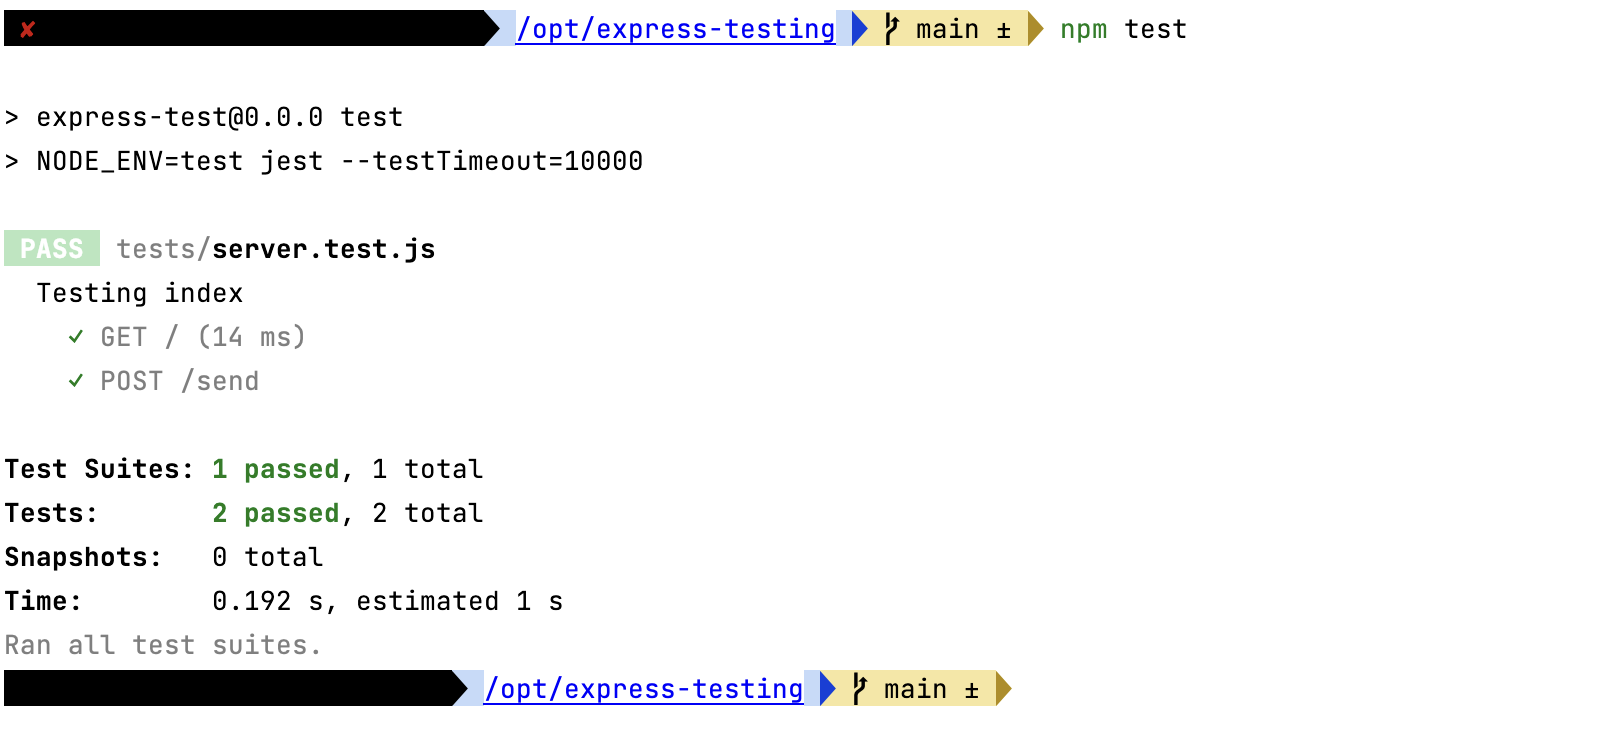
\includegraphics[width=0.75\textwidth]{img/testing/testing_npm_test_results.png}

\begin{itemize}
    \item 

Zer gertatuko litzateke janire@example.com ordez, maitane@example.com esperoko bagenu?

\begin{lstlisting}[language=JavaScript,numbers=none]
expect(res.body.data[1].email).toMatch("maitane@example.com")
\end{lstlisting}

Zein da jest exekutatzearen emaitza kasu honetan? (pantaila kaptura bat atera)

\end{itemize}

\item 
Orain beste erabiltzaile berri bat sartuko dugu, curl erabiliz:

\begin{lstlisting}[language=JavaScript,numbers=none]       
 curl -X POST http://localhost:4444/send/ -d "email=jota@gmail.com"

\end{lstlisting}


Ariketa: Nola aldatuko zenuke 10. ariketan egin dugun post() test-a 11. ariketan sartu dugun elementua ondo txertatu dela probatzeko?

\item 
Jarraian DELETE ruta probatuko dugu

Demagun hau dela uneko egoera:

\begin{verbatim}
  {"data":
    [{"id":52,"email":"test@example.com"}, 
     {"id":86,"email":"janire@example.com"},
      {"id":28,"email":"jota@gmail.com"}]}   


\end{verbatim}

Eta id:28-a duen elementua ezabatu nahi dugula. Lehenengo curl comandoaz probatuko dugu:

\begin{lstlisting}[language=JavaScript,numbers=none]
$ curl -X DELETE http://localhost:4444/destroy/28
{"data":    [{"id":52,"email":"test@example.com"},       {"id":86,"email":"janire@example.com"} ]
\end{lstlisting}

Ondo doala dirudi. 

Orain test bat prestatuko dugu. Horretarako, azken ID-a zein den kalkulatu ondoren (get() metodoaz) delete() bat exekutatuko dugu ID horren gainean)

\begin{lstlisting}[language=JavaScript,numbers=none]
it("DELETE /destroy/:id", async () => {
   const res = await request(url).get('/');
   const luzera = res.body.data.length
   // orduan azken elementua luzera -1 posizioan egongo da
   const id = res.body.data[luzera - 1].id
...
\end{lstlisting}

Jarraian id hori duen objektuaren ezabaketa ondo dabilela testeatuko dugu:

\begin{lstlisting}[language=JavaScript,numbers=none]
it("DELETE /destroy/:id", async () => {
   const res = await request(url).get('/');
   const luzera = res.body.data.length
   // orduan azken elementua luzera -1 posizioan egongo da
   const id = res.body.data[luzera - 1].id


   const response = await request(url).delete(`/destroy/${id}`);
   expect(response.type).toMatch(/json/)
   expect(res.statusCode).toBe(200);
   expect(response.body.data.length).toBe(luzera - 1)


})
\end{lstlisting}

Probatzeko:
\begin{verbatim}
$ npm test
\end{verbatim}

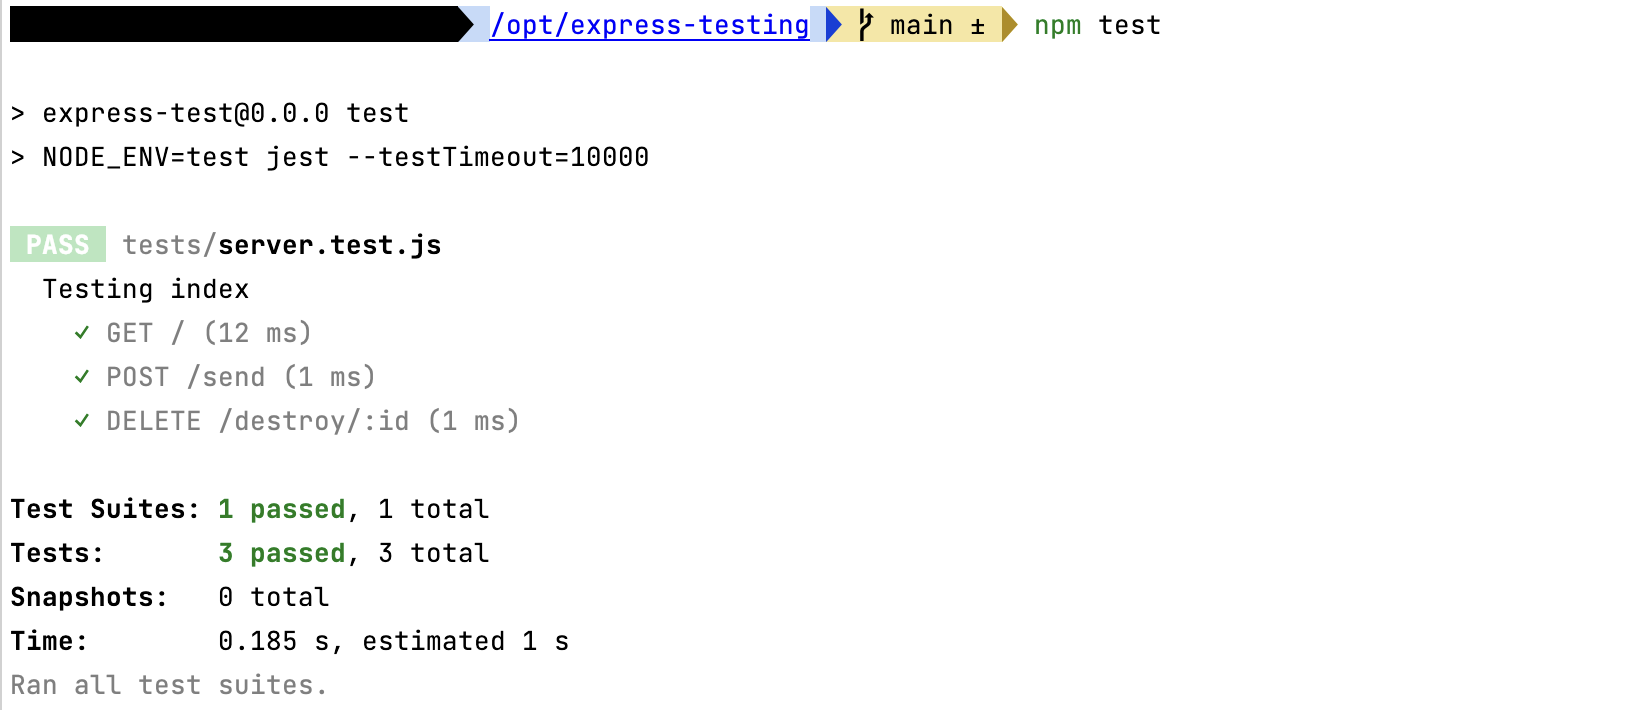
\includegraphics[width=0.75\textwidth]{img/testing/testing_npm_delete.png}

\item 
Ariketa: PUT ruta probatu

\begin{verbatim}
router.put("/update/:id", ....)    
\end{verbatim}


Horretarako:

\begin{itemize}
    \item 	13.1) Zein da CURL aplikazioaz probatzeko komandoa?
	(demagun lehenengo elementuaren email-a aldatu nahi dugula, test@example.com izan ordez, erabiltzaile@example.com izan dadila)

Erabili CURL aplikazioa lehenengo elementuaren emaila berriro test@example.com izan dadin.

\item 
13.2) Programatu test bat Jest eta SuperTest erabiliz (oinarritu zaitez 12. ariketan, oso-oso antzekoak baitira)

\end{itemize}
\end{enumerate}



